At each light injection point the duplex optical fibre will be held in place using a Fibre Support Structure (FSS). The purpose of the FSS is to ensure each fibre is aligned correctly as it points in towards the scintillator tanks and to provide a consistent 50mm curvature of the duplex optical fibre. Each FSS consists of 26 parts: 7 machined PTFE structural components; 7 passivated bolts; 9 passivated inserts; and two PTFE inserts. A photograph of a FSS with the lid open can be seen in figure \ref{fig:FFS}.

\begin{figure}[h]
    \centering
    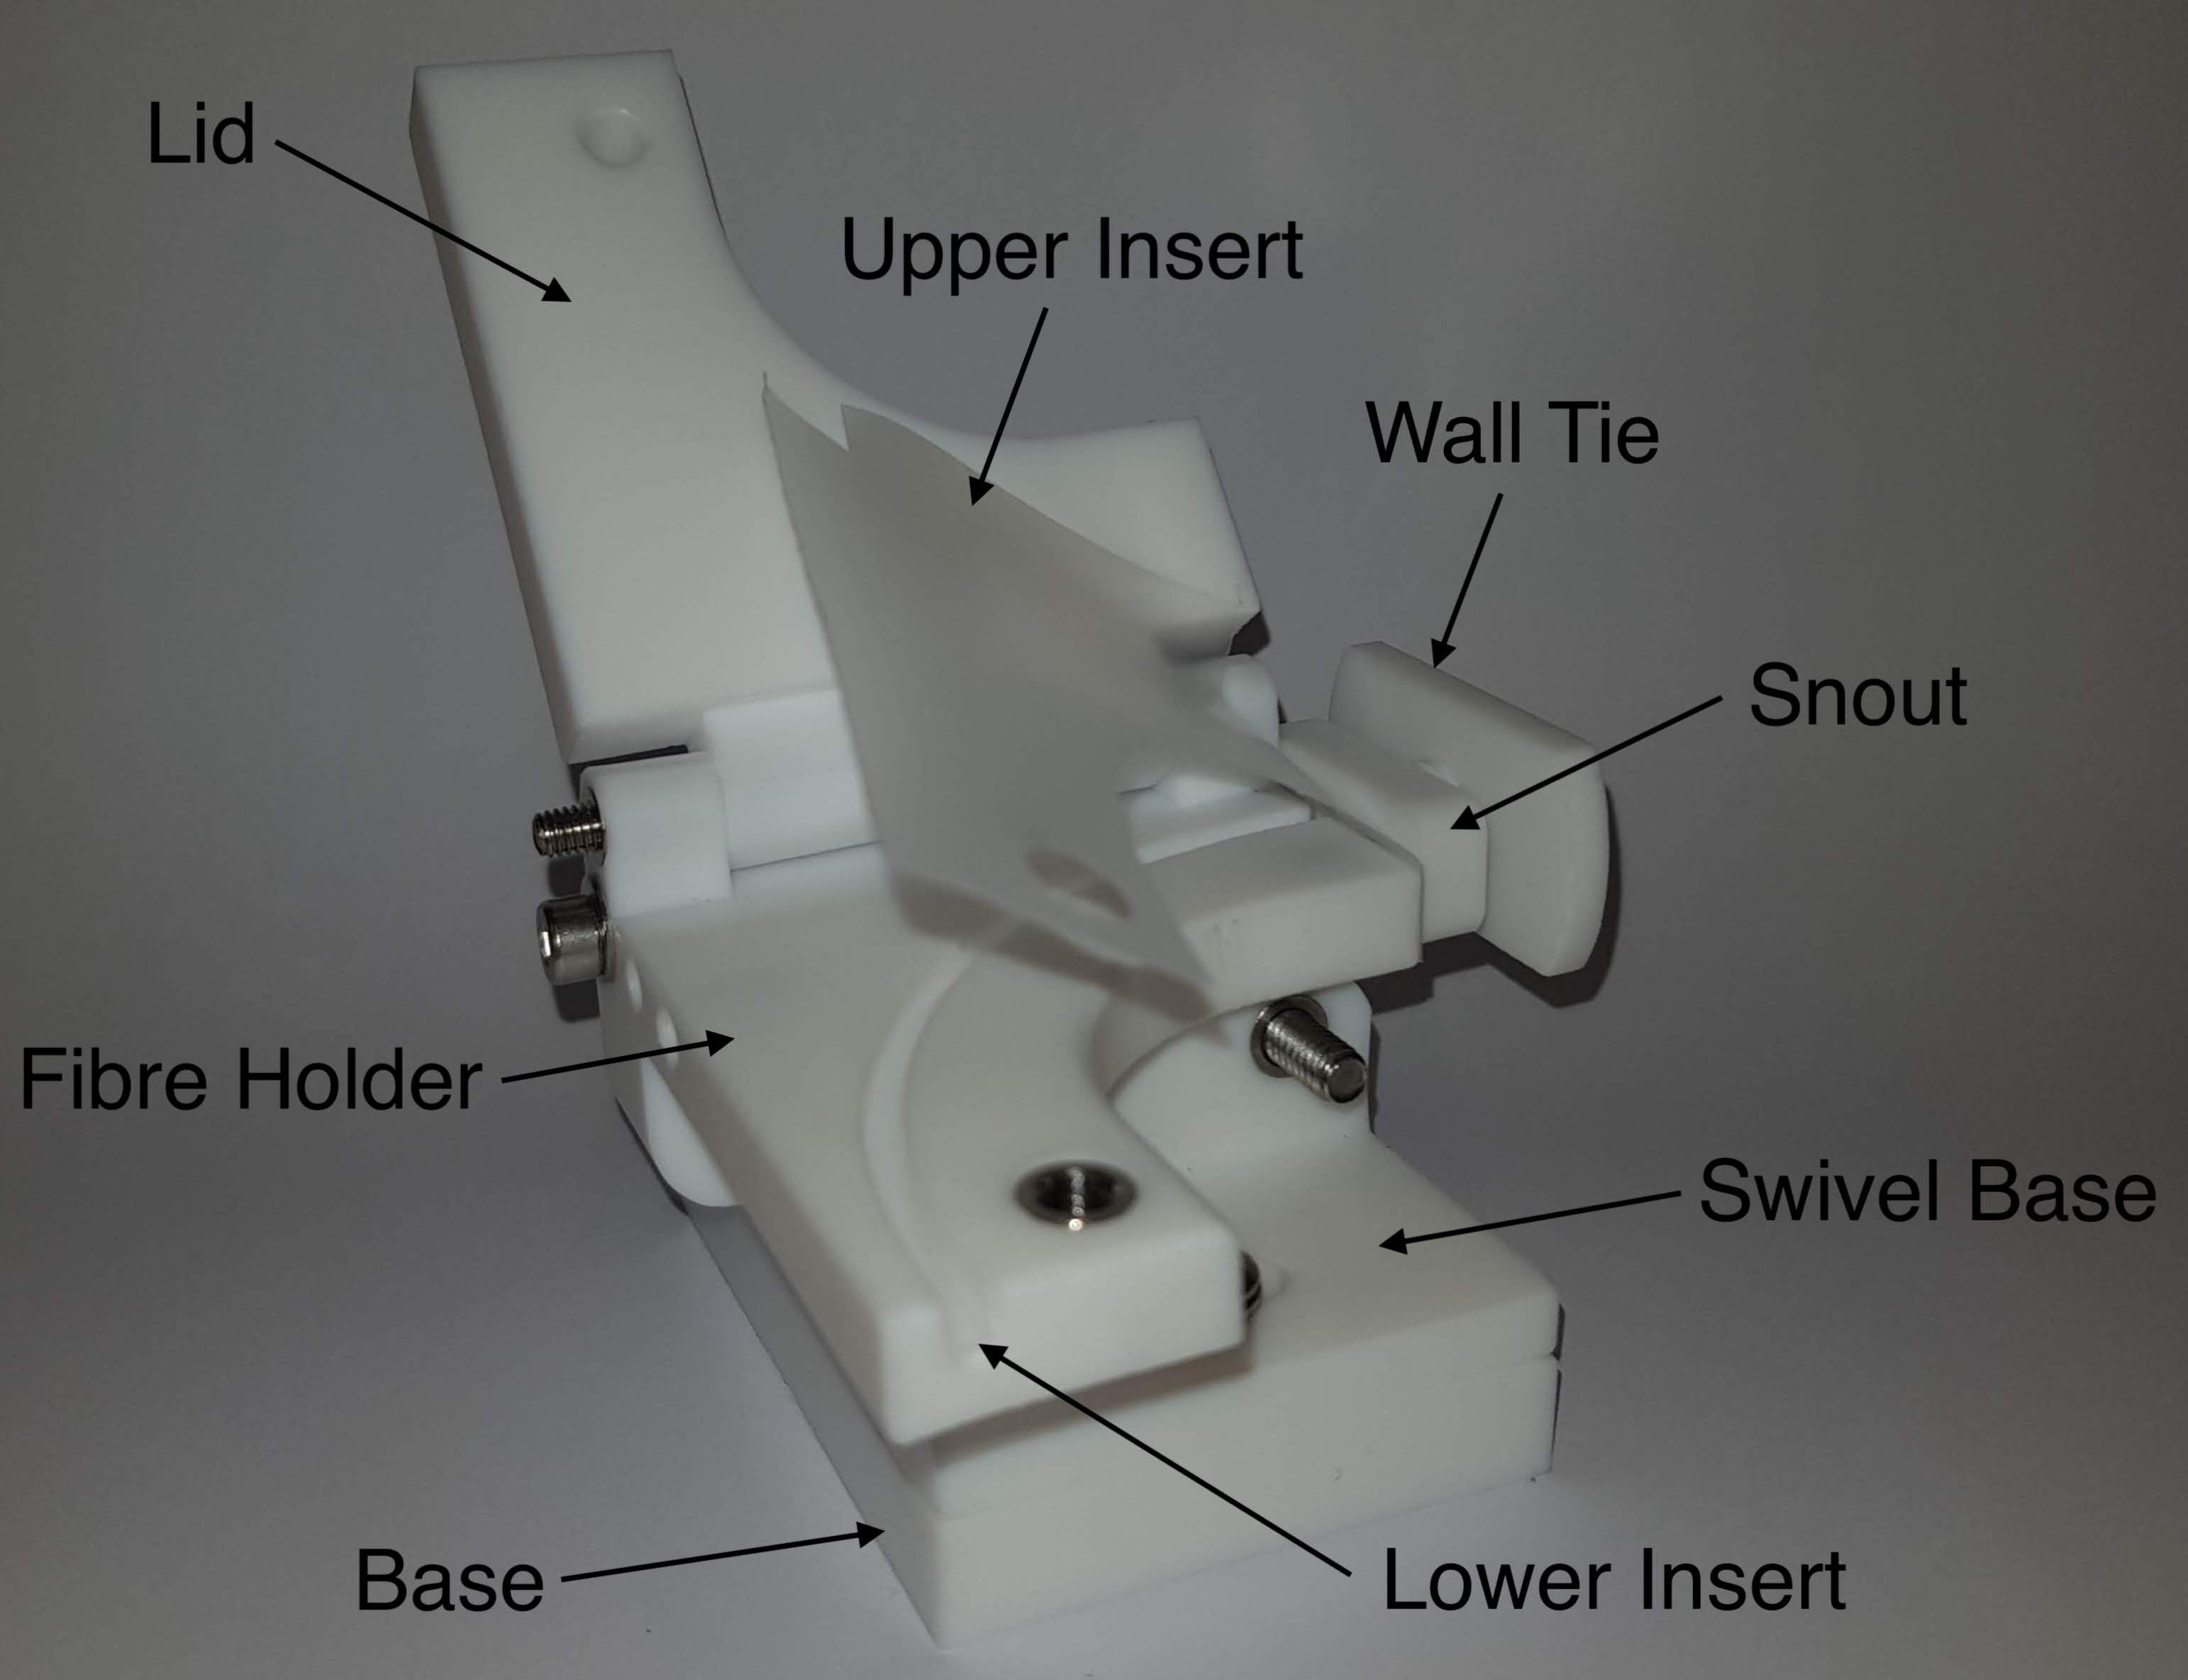
\includegraphics[width=0.7\textwidth, angle=0]{Figures/FSS.jpg}
    \caption{A photograph of one of the FSS with the lid open. The 8 key components of the FSS are labelled repectively}
    \label{fig:FFS}
\end{figure}

\section{Testing}
After the manufacturing of the FSS's was completed a random selection of 6 FSS's were sent to the Boulby Underground Laboratory for radioactive screening. The results from the screening have been compared to the estimated activities of the OD components in table \ref{table:radio-nuc}.  
\begin{table}[h!]
\centering
\begin{tabular}{|c|c|c|c|c|c|c|c|} 
    \hline
    Outer Detector Components & Mass / kg & $U_e^{238}$ & $U_l^{238}$ & $Th_e^{232}$ & $Th_l^{232}$ & $Co^{60}$ & $K^{40}$ \\
    & & \multicolumn{6}{c|}{Activity (mBq/kg)} \\
    \hline
    Outer Detector Tanks & 3200 & 0.16 & 0.39 & 0.02 & 0.06 & 0.04 & 5.36 \\
    \hline
    Liquid Scintillator & 17600 & 0.01 & 0.01 & 0.01 & 0.01 & 0.00 & 0.00 \\
    \hline
    Outer Detector PMTs & 205 & 570 & 470 & 395 & 388 & 0.00 & 534 \\
    \hline
    OD PMT Supports & 770 & 1.20 & 0.27 & 0.33 & 0.49 & 1.60 & 0.40 \\
    \hline
    Fibre Support Structure & 0.350 & 31 & 3.0 & 6.0 & 3.0 & 0.5 & 330 \\
    \hline
\end{tabular}
\caption{Estimated activities of the radio-nuclides present in the OD components are presented with the results from the screening of the FSSs at Boulby Underground Laboratory. A comprehensive list of the estimated activities for the rest of the detector can be found in the LZ-TDR \cite{LZTDR}.}
\label{table:radio-nuc}
\end{table}
In comparison with the OD components, the results show relatively large activities in potassium-40 in the screened sample. This could be due to environmental containment's which remained on the sample after being wiped with propan-2-ol. Before the next set of samples are sent for screening, they will be cleaned using the procedure that will be implemented before installation at the experiment. Results from the two screenings will be compared to ensure that the high levels of potassium-40 is due to environmental containment's and not from containment's within the PTFE material.

\section{Fibre support structure - insert development}\label{sec:FSSID}
After the construction a duplex optical fibre was place into the FSS and it was found that the PTFE material which the structural components were produced from didn't grip the fibre when a small force was applied. In this section, the series of tests and the components produced to resolve this problem will be discussed. 

\subsection{Insert description}
Two inserts were designed to fit between the fibre and the PTFE material. The templates for the inserts can be seen in figure \ref{fig:inserts}. The upper insert is placed in groove of the fibre holder below the fibre and lower insert is placed between the lid of the FFS and the fibre holder component, seen in figure \ref{fig:FFS}. Both inserts are attached to the FSS using bolts which are used to attach the snout piece to the fibre holder.

\begin{figure}[h!]
    \centering
    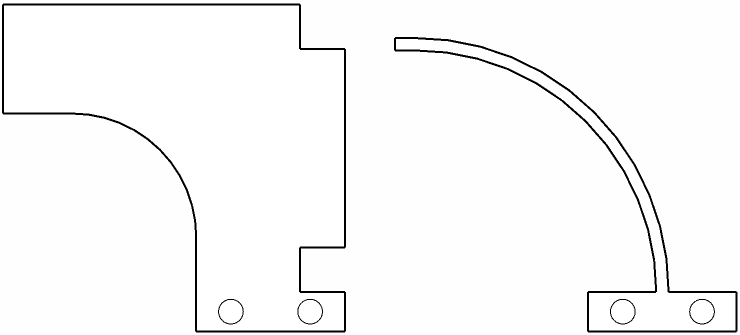
\includegraphics[width=0.7\textwidth]{Figures/Slip_inserts.jpg}
    \caption{Inserts are designed to fit between the duplex fibre and the PTFE components of the FSS. The upper insert is placed between the FSS lid and the fibre (left). The lower insert is placed between the fibre and FSS fibre holder, sitting inside the groove (right).}
    \label{fig:inserts}
\end{figure}

\subsection{Testing}
The force required to induce creep in the fibre when being held by the FSS was tested using the apparatus in figure \ref{fig:FPTT_Test_Stand}. Variations in the arrangement of the inserts were tested in varying moisture conditions. The arrangements tested were: no inserts (A); one upper insert with no lower insert (B); two upper inserts with no lower insert (C); and one upper insert with one lower insert (D). The moisture conditions were varied between: "dry" where no water was used; "drip" where de-ionised water was pipetted down the groove of the fibre holder; and "submersion" where the entire FSS was submerged in de-ionised water to simulate how the FSS would perform in the water tank of the OD. Each of the insert arrangements were tested under dry conditions and then the best two were tested under more moist conditions. The results from the testing can be found in table \ref{table:FPTT} and are displayed in figure \ref{fig:FPTT_plot}. 

\subsection{Results}
In the test arrangement D performed best in comparison with the other arrangements under the varied moisture conditions and it would be recommended that this arrangement is used during the running of the experiment. It can also be seen that the force required to pull the fibre from the FSS should be greater than any force encountered on the fibres. 

\begin{figure}[h]
    \centering
    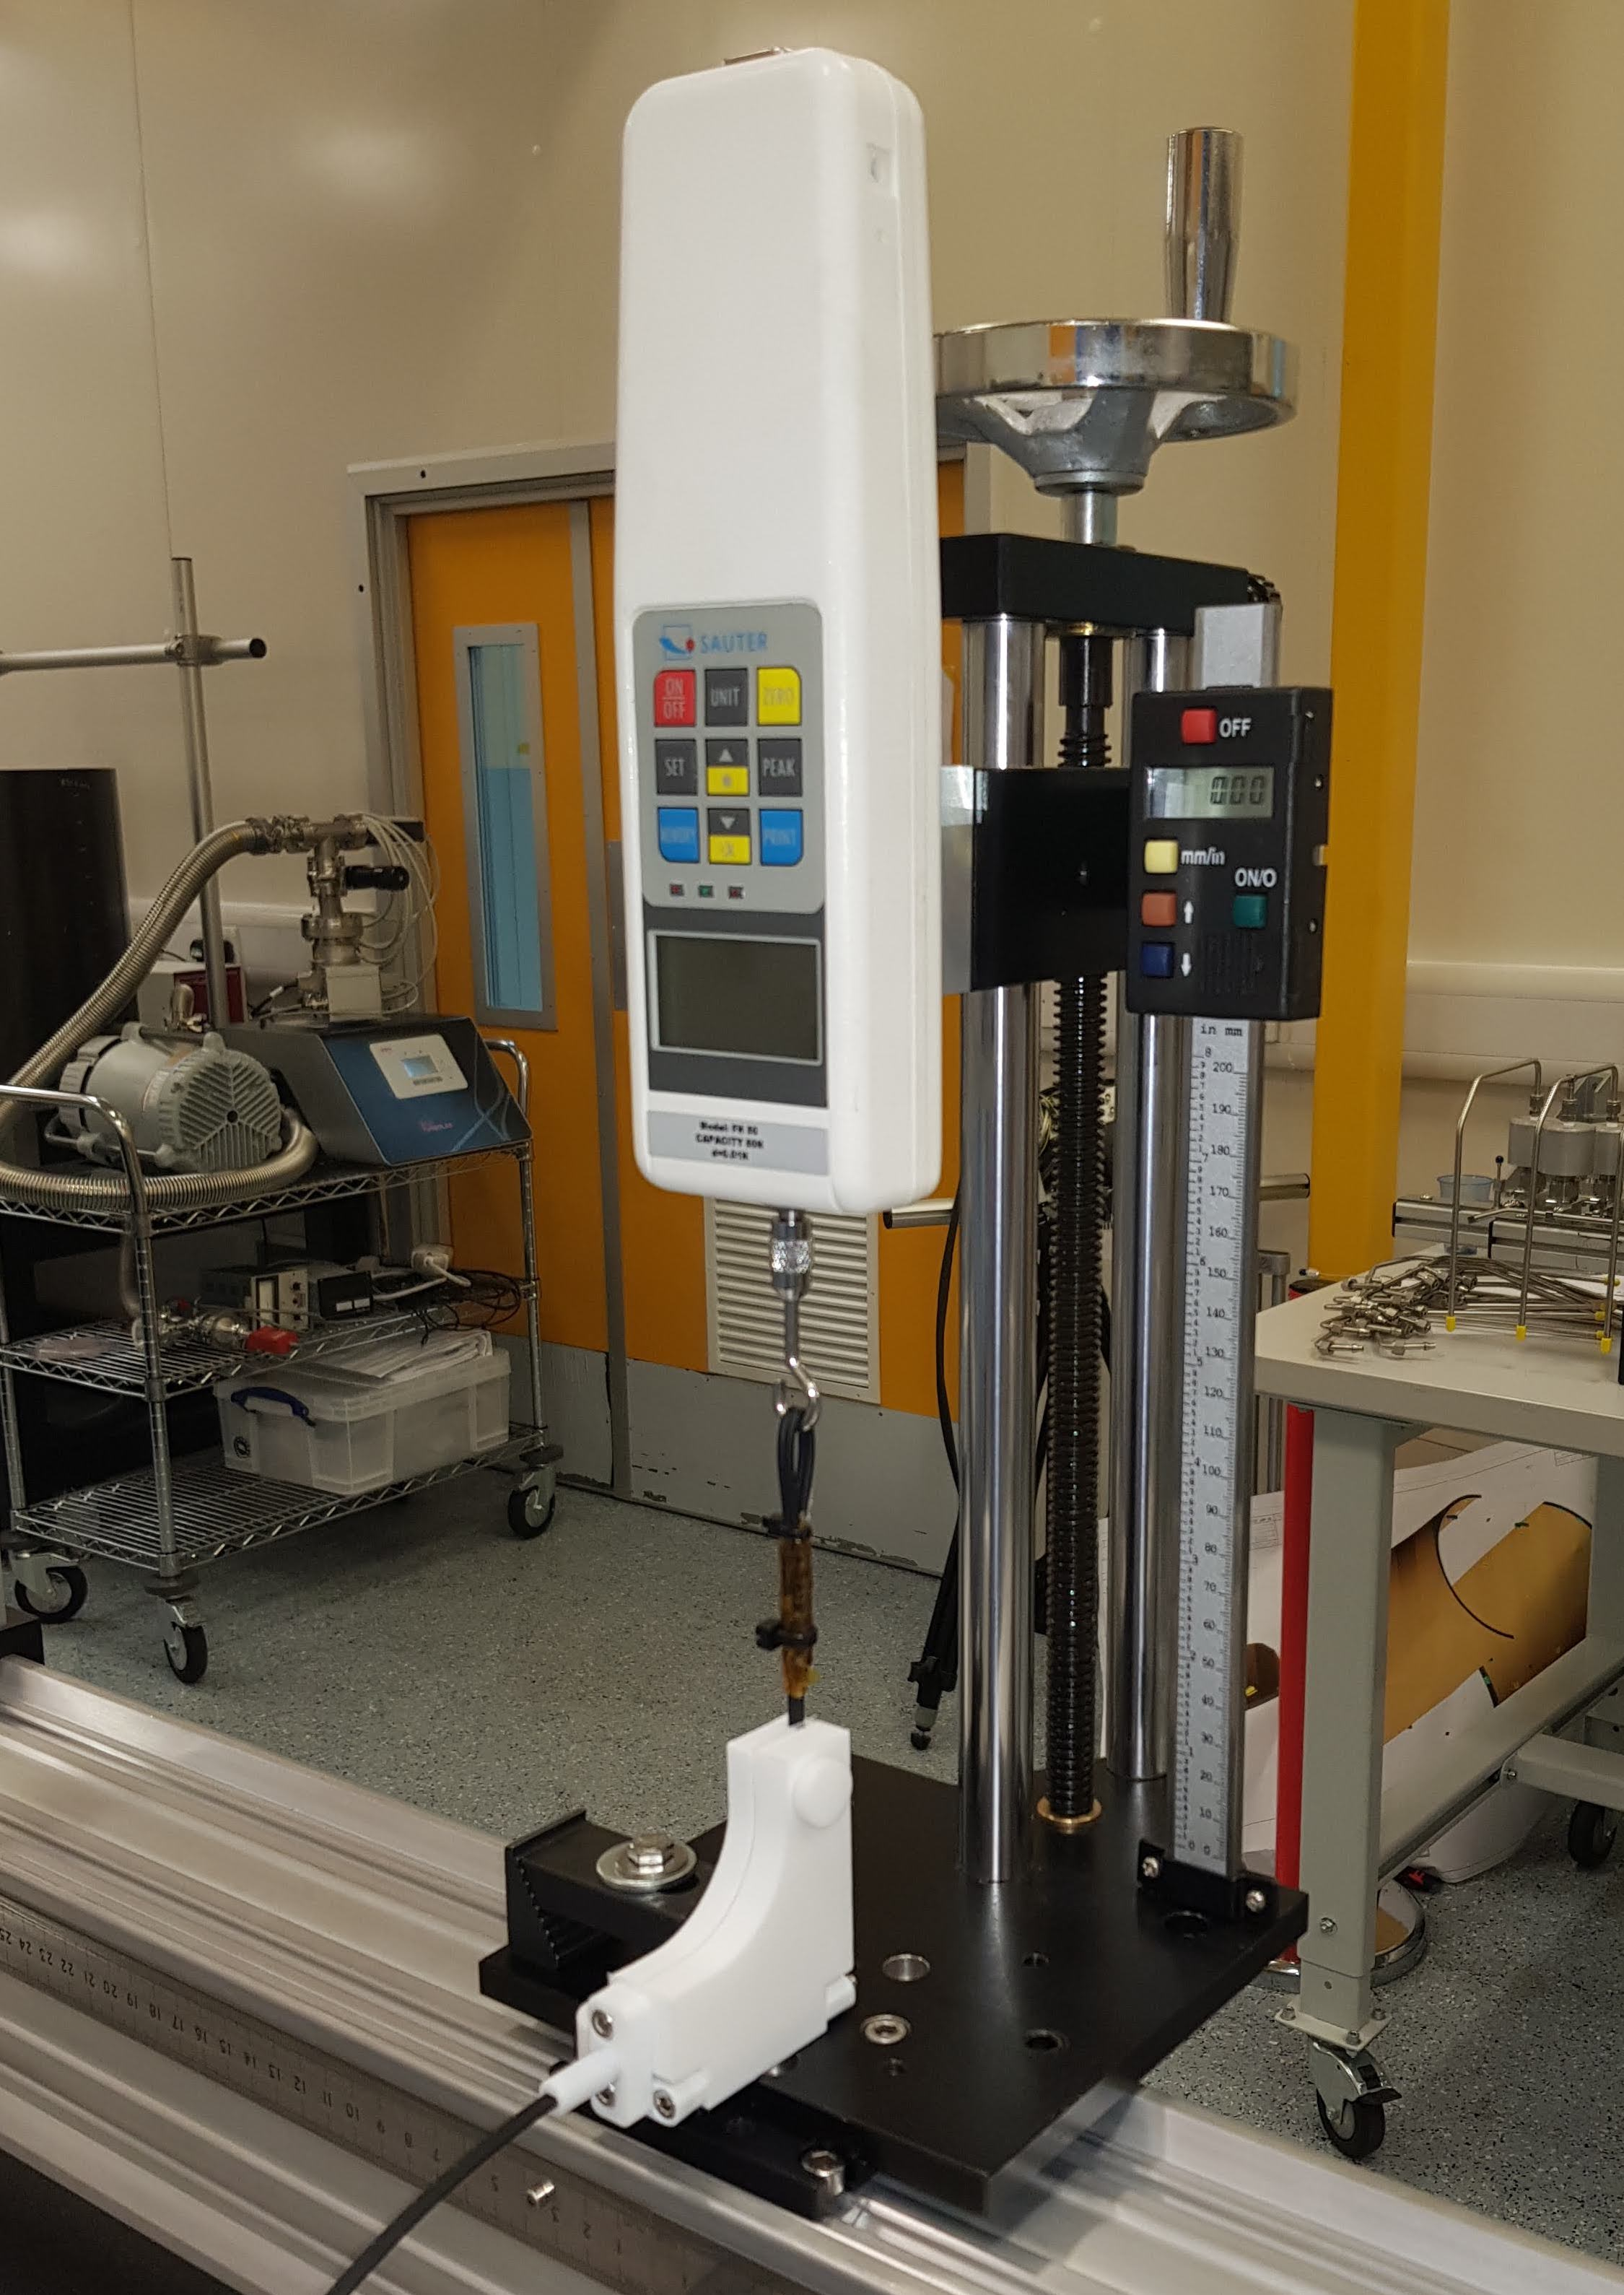
\includegraphics[width=0.6\textwidth]{Figures/FPTT_Test_Stand.jpg}
    \caption{Photograph showing the setup of the apparatus used in the fibre pull through test.}
    \label{fig:FPTT_Test_Stand}
\end{figure}

\begin{table}[h!]
\centering
    \begin{tabular}{c|c|c|c|} 
        \cline{2-4}
        & \multicolumn{3}{|c|}{Moisture Condition}
        \cr. \cline{2-4}
        \hline
        \multicolumn{1}{|c|}{Insert Arrangement} &Dry / N& Drip / N& Submersion / N\\
        \hline
        \multicolumn{1}{|c|}{A} & $6.4 \pm 0.2$ & - & - \\
        \multicolumn{1}{|c|}{B} & $12.0 \pm 0.3$ & - & - \\
        \multicolumn{1}{|c|}{C} & $13.4 \pm 0.5$ & $12.0 \pm 0.3$ & - \\
        \multicolumn{1}{|c|}{D} & $17.8 \pm 1.1$ & $18.4 \pm 1.1$ & $16.4 \pm 0.3$ \\
        \hline
    \end{tabular}
\caption{In this table, the force required to induce creep in the fibre under varying moisture conditions and insert arrangement.}
\label{table:FPTT}
\end{table}

\begin{figure}[h]
    \centering
    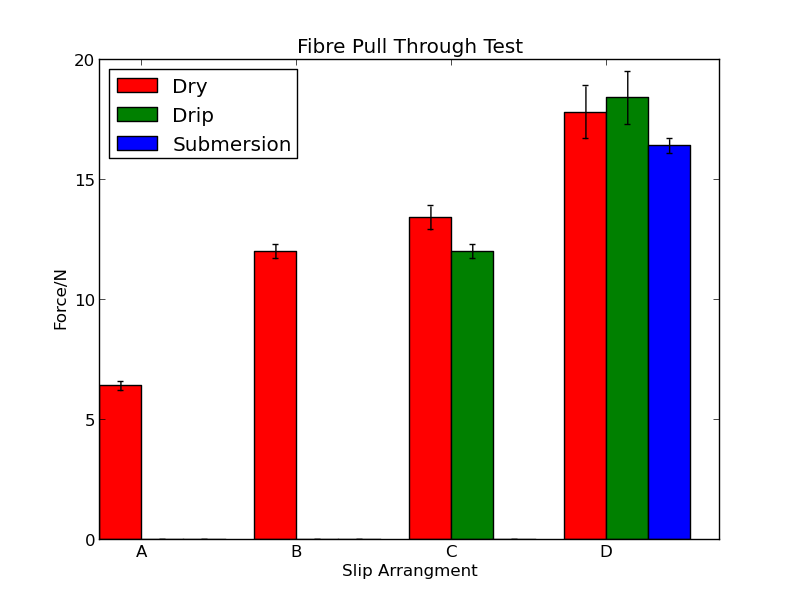
\includegraphics[width=0.7\textwidth]{Figures/FPTT_plot.png}
    \caption{Plot showing the force required to move a fibre under varied moisture conditions with different slip arrangements.}
    \label{fig:FPTT_plot}
\end{figure}

In the test arrangement D performed best in comparison with the other arrangements under the varied moisture conditions and it would be recommended that this arrangement is used during the running of the experiment. It can also be seen that the force required to pull the fibre from the FSS will be greater than any force which could be generated from waves oscillating during the filling of the water tank. 
